\documentclass[jou,floatsintext]{apa6}
\usepackage{lmodern}
\usepackage{amssymb,amsmath}
\usepackage{ifxetex,ifluatex}
\usepackage{fixltx2e} % provides \textsubscript
\ifnum 0\ifxetex 1\fi\ifluatex 1\fi=0 % if pdftex
  \usepackage[T1]{fontenc}
  \usepackage[utf8]{inputenc}
\else % if luatex or xelatex
  \ifxetex
    \usepackage{mathspec}
  \else
    \usepackage{fontspec}
  \fi
  \defaultfontfeatures{Ligatures=TeX,Scale=MatchLowercase}
\fi
% use upquote if available, for straight quotes in verbatim environments
\IfFileExists{upquote.sty}{\usepackage{upquote}}{}
% use microtype if available
\IfFileExists{microtype.sty}{%
\usepackage{microtype}
\UseMicrotypeSet[protrusion]{basicmath} % disable protrusion for tt fonts
}{}
\usepackage{hyperref}
\hypersetup{unicode=true,
            pdftitle={Trait plasticity and covariance along a continuous soil moisture gradient},
            pdfauthor={J. Grey Monroe, Haoran Cai, \& David L. Des Marais},
            pdfkeywords={drought, function-valued traits, Brachypodium, evolutionary constraint, phenotypic plasticity, non-linearity},
            pdfborder={0 0 0},
            breaklinks=true}
\urlstyle{same}  % don't use monospace font for urls
\usepackage{graphicx,grffile}
\makeatletter
\def\maxwidth{\ifdim\Gin@nat@width>\linewidth\linewidth\else\Gin@nat@width\fi}
\def\maxheight{\ifdim\Gin@nat@height>\textheight\textheight\else\Gin@nat@height\fi}
\makeatother
% Scale images if necessary, so that they will not overflow the page
% margins by default, and it is still possible to overwrite the defaults
% using explicit options in \includegraphics[width, height, ...]{}
\setkeys{Gin}{width=\maxwidth,height=\maxheight,keepaspectratio}
\IfFileExists{parskip.sty}{%
\usepackage{parskip}
}{% else
\setlength{\parindent}{0pt}
\setlength{\parskip}{6pt plus 2pt minus 1pt}
}
\setlength{\emergencystretch}{3em}  % prevent overfull lines
\providecommand{\tightlist}{%
  \setlength{\itemsep}{0pt}\setlength{\parskip}{0pt}}
\setcounter{secnumdepth}{0}
% Redefines (sub)paragraphs to behave more like sections
\ifx\paragraph\undefined\else
\let\oldparagraph\paragraph
\renewcommand{\paragraph}[1]{\oldparagraph{#1}\mbox{}}
\fi
\ifx\subparagraph\undefined\else
\let\oldsubparagraph\subparagraph
\renewcommand{\subparagraph}[1]{\oldsubparagraph{#1}\mbox{}}
\fi

%%% Use protect on footnotes to avoid problems with footnotes in titles
\let\rmarkdownfootnote\footnote%
\def\footnote{\protect\rmarkdownfootnote}


  \title{Trait plasticity and covariance along a continuous soil moisture gradient}
    \author{J. Grey Monroe\textsuperscript{1}, Haoran Cai\textsuperscript{2}, \& David L. Des Marais\textsuperscript{2,3}}
    \date{}
  
\shorttitle{Function-valued drought extremes}
\affiliation{
\vspace{0.5cm}
\textsuperscript{1} Department of Plant Sciences, University of California at Davis, Davis, USA\\\textsuperscript{2} Department of Civil and Environmental Engineering, Massachusetts Institute of Technology, Cambridge, MA, USA\\\textsuperscript{3} The Arnold Arboretum of Harvard University. Boston, MA, USA}
\keywords{drought, function-valued traits, Brachypodium, evolutionary constraint, phenotypic plasticity, non-linearity}
\usepackage{csquotes}
\usepackage{upgreek}
\captionsetup{font=singlespacing,justification=justified}

\usepackage{longtable}
\usepackage{lscape}
\usepackage{multirow}
\usepackage{tabularx}
\usepackage[flushleft]{threeparttable}
\usepackage{threeparttablex}

\newenvironment{lltable}{\begin{landscape}\begin{center}\begin{ThreePartTable}}{\end{ThreePartTable}\end{center}\end{landscape}}

\makeatletter
\newcommand\LastLTentrywidth{1em}
\newlength\longtablewidth
\setlength{\longtablewidth}{1in}
\newcommand{\getlongtablewidth}{\begingroup \ifcsname LT@\roman{LT@tables}\endcsname \global\longtablewidth=0pt \renewcommand{\LT@entry}[2]{\global\advance\longtablewidth by ##2\relax\gdef\LastLTentrywidth{##2}}\@nameuse{LT@\roman{LT@tables}} \fi \endgroup}
\newcommand{\beginsupplement}{\setcounter{table}{0}  \renewcommand{\thetable}{S\arabic{table}} \setcounter{figure}{0} \renewcommand{\thefigure}{S\arabic{figure}}}

\authornote{

Correspondence concerning this article should be addressed to J. Grey Monroe, 262 Robbins Hall, UC Davis, One Shields Ave, Davis CA 95616. E-mail: \href{mailto:greymonroe@gmail.com}{\nolinkurl{greymonroe@gmail.com}}}

\abstract{
Water is perhaps the greatest environmental determinant of plant yield and fitness, yet our understanding of plant-water relations is limited because it is primarily informed by experiments that have treated soil moisture variability as two simple discrete levels - wet and dry - rather than a continually varying environmental gradient. Here we used experimental and statistical methods based on function-valued traits to study responses to continuously varying soil moisture gradient in a suite of physiological and morphological traits in two species and multiple genotypes of the model grass \textit{Brachypodium}. We find that the majority of traits exhibit non-linear responses to soil moisture variability. We also observe differences in the shape of these non-linear responses between traits, species, and genotypes. Emergent phenomena arise from this variation including changes in trait correlations and evolutionary constraints as a function of soil moisture. These results point to the importance of considering non-linearity in plant-water relations to predict outcomes of adaptation to changing climates.

}

\begin{document}
\maketitle

\hypertarget{introduction}{%
\section{Introduction}\label{introduction}}

For plants, soil water availability is one of the most important environmental factors in ecology and agriculture, acting as a major determinant of fitness and yield (Juenger 2013; Greenham \emph{et al.} 2017). Considerable interest and effort have been placed on studying plant responses to drought, often defined conceptually and experimentally as an environmental condition of abnormally elevated aridity resulting in decreased plant performance (Passioura 1996). Most of the vast research on drought responses and tolerance strategies, including in \emph{Brachypodium}, the focal system of this work, has been limited to comparisons between discrete soil water levels - control and water-limited (Des Marais \emph{et al.} 2012; Edwards \emph{et al.} 2012; El-Soda \emph{et al.} 2014; Vasseur \emph{et al.} 2014; Greenham \emph{et al.} 2017). Yet soil moisture as an environmental factor is complex and multidimensional, with fluctuations varying continuously in timing, duration, and degree. Here we investigate trait responses to one important dimension of soil moisture variability - degree - with experimental and statistical approaches treating soil moisture content as a continuous variable rather than a set of fixed levels.

The limited extent to which continuous environmental variables have been studied is not unique to investigations of plant responses to soil moisture. Recent decades have seen increased appreciation for modeling traits as mathematical functions of continuous variables across diverse organisms (Pettay \emph{et al.} 2008; Rocha and Klaczko 2012; Mason \emph{et al.} 2020), a wide range of traits (Robinson \emph{et al.} 2009; McGuigan \emph{et al.} 2010; Stinchcombe \emph{et al.} 2010), and numerous components of the environment (Brommer \emph{et al.} 2008; McGuigan 2009; Pearse \emph{et al.} 2019). This burgeoning interest in the importance of \enquote{function-valued traits} has evolved from a call-to-arms to a field experiencing rapid theoretical and empirical advances (Kirkpatrick and Heckman 1989; Kingsolver \emph{et al.} 2001; Griswold \emph{et al.} 2008; Stinchcombe \emph{et al.} 2012; Goolsby 2015; Gomulkiewicz \emph{et al.} 2018). For plant biologists this presents a compelling framework for gaining a deeper understanding of plant adaptations to the environment.

A deep body of literature aims to understand the traits and strategies used by plants to acclimate to variable soil water content. Quantitative genetic variation in myriad drought resistance traits have been observed in natural populations and laboratory model systems. In particular, natural populations of Brassicaceae species (including \emph{Arabidopsis thaliana}) and \emph{Brachypodium} harbor variation both constitutive and inducible traits mediating plant-water relations, including water use efficiency (Des Marais \emph{et al.} 2012, 2017; Edwards \emph{et al.} 2012; Greenham \emph{et al.} 2017), production of compatible osmolytes (Kesari \emph{et al.} 2012; Des Marais \emph{et al.} 2017), leaf anatomy (Skirycz \emph{et al.} 2011; Verelst \emph{et al.} 2013; Dittberner \emph{et al.} 2018), root-shoot biomass partitioning (Des Marais \emph{et al.} 2012, 2017), and many others (Verslues and Juenger 2011; Edwards \emph{et al.} 2012; Juenger 2013; Luo \emph{et al.} 2016; Yarkhunova \emph{et al.} 2016; Lenk \emph{et al.} 2019). Among the numerous plant traits that can and have been measured, few have been studied more extensively than specific leaf area (SLA - often reported as it's inverse, leaf mass per area or LMA). SLA provides a description of leaf architecture that is central to the leaf economics spectrum, a theory which seeks to explain variation in leaf physiological strategies, from more conservative (low SLA) to more productive (high SLA) (Wright \emph{et al.} 2004). In the context of drought stress, it is intuitive that low SLA might be adaptive as lower leaf surface area is expected to reduce water loss through transpiration. In several cases, reductions in SLA have been reported under drought conditions (Casper \emph{et al.} 2001).

Despite abundant evidence of natural variation in organism-environment interaction, little is known as to how trait covariance changes across continuous environmental gradients (but see Robinson \emph{et al.} 2009). Describing this structure is important as trait variances and covariances can result in differential evolutionary constraints in alternative environments. For example, if total genetic variance in trait space changes depending on the environment, then the capacity to respond to selection will vary accordingly, with reduced responses to selection under conditions where trait variation is lower and vice versa. Similarly, if trait covariances depend on environment, conditions which increase trait covariances may limit evolutionary potential across a range of environments by reducing the effective axes of variation (Levins 1968; Via and Lande 1985; Kingsolver and Gomulkiewicz 2003; Gomulkiewicz \emph{et al.} 2018). These phenomena are made more complex by the possibility that the relationship between trait variances and covariances with the environment may be non-linear. Investigating complexities of genetic architecture is therefore needed for developing more complete quantitative predictions of evolvability in rapidly changing environments. Fortunately, advances have been made in statistical methods to reduce the dimensionality of genetic variance covariance matrices and produce meaningful summaries describing evolutionary constraints (Houle 1992; Blows 2007; Kirkpatrick 2009; Kingsolver \emph{et al.} 2015).

In this study we combined these approaches with function-valued trait analyses to investigate trait plasticity, covariance and evolutionary constraints across soil moisture gradients. We model trait responses to a continuous gradient of soil moisture for a range of genotypes of two species of the model grass genus \emph{Brachypodium}. Because the shapes of trait responses cannot necessarily be known \emph{a priori}, we use model selection among linear and non-linear environmental predictors to estimate the response function for each trait. We then estimate genotype means at different levels of soil moisture and compute the variance-covariance parameters for all traits. Finally, we ask whether patterns of variance and covariance in drying-responsive traits in \emph{Brachypodium} species may lead to variation in evolutionary constraint as a function of soil moisture.

\hypertarget{materials-and-methods}{%
\section{Materials and Methods}\label{materials-and-methods}}

\hypertarget{genotypes-and-species}{%
\subsubsection{Genotypes and species}\label{genotypes-and-species}}

\emph{Brachypodium} is a model genus for the genetics and genomics of C3 grasses (Brkljacic \emph{et al.} 2011). In this work we studied natural variation between and among two species of \emph{Brachypodium}: the annual \emph{B. distachyon} and the perennial \emph{B. sylvaticum}. Both species are endemic to Eurasia, with \emph{B.distachyon} more prevalent in seasonally dry habitats in Southern Europe, North Africa, and the Middle East, and \emph{B. sylvaticum} more widely distributed throughout Eurasia (Catalan \emph{et al.} 2016) (Figure \ref{fig:maps}).

Five genotypes of each species were studied to characterize patterns of variation in plant traits across an environmental gradient: \emph{Brachypodium distachyon} inbred lines ABR2, Adi-10, Bd21, Bd3-1, and Koz-1 and \emph{Brachypodium sylvaticum} inbred lines Ain-1, Ast-1, Kry-1, Osl-1, Vel-1. For each species, these genotypes represent a range of geographical origins and phenotypic diversity (Steinwand \emph{et al.} 2013; Des Marais \emph{et al.} 2017). Both species are self-compatible and each of the lines used here have been maintained as inbred lines for greater than six generations (Vogel \emph{et al.} 2009; Steinwand \emph{et al.} 2013); as such, experimental replicates may be considered nearly homozygous.

\hypertarget{plant-growth-and-dry-down-experiment}{%
\subsubsection{Plant growth and dry down experiment}\label{plant-growth-and-dry-down-experiment}}



\begin{figure*}[!h]
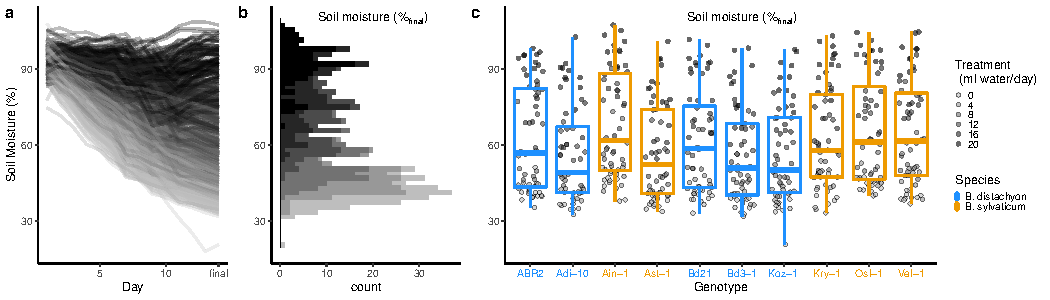
\includegraphics[width=\textwidth]{../Figures/DryDown_lines} \caption{\textbf{Effect of the experimental dry down on soil water content.} (A) Time series of gravimetric soil moisture for all pots during the 14-day dry down period. (B) Distribution of final (day 14) soil moisture content across all pots. The data are distinguished by color according to the watering treatment. (C) Final soil moisture content by genotype.}\label{fig:drydown}
\end{figure*}

Plant growth and experimental soil dry down were performed in the greenhouses of the Arnold Arboretum of Harvard University. To synchronize germination across genotypes within each species, seeds were placed on damp filter paper in the dark at 4°C for 14 days prior to planting. To synchronize the developmental stage at the timing of the drought treatments between the two species, \emph{B. sylvaticum} seeds were planted thirteen days before \emph{B. distachyon} (Oct 7 and 20, 2015, respectively). For each genotype, 1200 seeds were planted two to a pot and were subsequently thinned to one plant, for a total of 600 experimental plants in a randomized block design. All plants germinated within four days of sowing. Individual seeds of plants were sown in Greens Grade Profile porous ceramic rooting media (Profile Products, Buffalo Grove, IL, USA) in Deepot D40H Conetainers (650mL; Stuewe \& Sons. Tangent, OR, USA) and grown at 25°C/20°C days/nights. Ambient sunlight was supplemented to 1000 umol/m2/s for 12hr/day.

Dry down treatments began 29 and 42 days after sowing (DAS) for \emph{B. distachyon} and \emph{B. sylvaticum}, respectively. Because the harvesting was divided over five consecutive days (see section below), plants were split into five equal harvest cohorts, with each cohort containing equal numbers of each watering treatment to avoid confounding harvest day with soil moisture content. Thus, though each consecutive cohort differed in age by a single day, each experienced the dry down treatment for the same amount of time. Nevertheless, we expected the difference in age between harvest cohorts to potentially impact trait expression and we therefore included harvest day (cohort) as a covariate in subsequent models. To generate a continuous gradient of final soil moisture by the end of the dry down period, plants were split into five watering treatments, receiving approximately 0, 4, 8, 12, 16, or 20 ml of water per day for 14 days. Prior to initiating the experiment pots were weighed with dry soil (\(mass_{dry}\)) and field capacity (\(mass_{max}\)) at the beginning of the experiment. These measurements provide the basis for calculating the gravimetric soil moisture content on each day and at the conclusion of the experiment. During the course of the dry down experiment, soil moisture content was calculated during the morning of day \(d\) for each pot as \(mass_d/(mass_{max}-mass_{dry})\).

\hypertarget{plant-harvesting-and-phenotyping}{%
\subsubsection{Plant harvesting and phenotyping}\label{plant-harvesting-and-phenotyping}}

To characterize phenotypic responses to our simulated drought, we measured a suite of developmental and physiological traits. Plants were harvested in five cohorts over five days. Each day, half of the sampled plants were harvested for above and below ground biomass, total above ground green area, \(\delta C_{13}\), N content, C content. The other half were harvested and assessed for specific leaf area (SLA) and relative water content (RWC). Above ground biomass was measured after drying leaf material overnight at 60°C. Below ground biomass was measured after washing the soil matrix from roots and drying them overnight at 60°C. Above ground leaf area was estimated by laying plants flat between plates of clear plexiglass and imaging with a Nikon 5300 digital camera at a fixed distance with a 35mm Nikkor lens. Total green pixels were counted for each image with Easy Leaf Area with settings shown in Figure \ref{fig:leafarea}. SLA was calculated by scanning the two youngest fully emerged leaves. Leaf area was calculated from these same images using Easy Leaf Area. Above and belowground biomass was measured after leaves were dried and SLA was calculated as \(leaf\ area / biomass_{dry}\). Leaf tissues for \(\delta C_{13}\), \(\delta N_{15}\), nitrogen (hereafter \enquote{N}) content, and carbon (hereafter \enquote{C}) content were ground to a fine powder and processed by the UC Davis Stable Isotope Facility. These leaves were also used to calculate RWC. Prior to drying, fresh leaves were weighed (\(biomass_{fresh}\)) and then submerged under water in 15mL falcon tubes for several hours. They were then weighed (\(biomass_{turgid})\), oven-dried overnight, and weighed again (\(biomass_{dry}\)). RWC was calculated as \((biomass_{fresh}-biomass_{dry})/(biomass_{turgid}-biomass_{dry})\)\}.

\begin{table*}[tbp]
\begin{center}
\begin{threeparttable}
\caption{\label{tab:models}Model selection. *** = predictor variable p < 1e-5, ** = predictor variable p < 1e-3, * = predictor variable p < 0.5, - = predictor variable included in selected model but p > 0.05. H = harvest day, S = species, G = genotype, E = final soil moisture, E\textasciicircum{}2 = quadratic parameter, ns(E) = 2nd degree natural spline parameter}
\scriptsize{
\begin{tabular}{ccccccccc}
\toprule
 & \multicolumn{1}{c}{G} & \multicolumn{1}{c}{E} & \multicolumn{1}{c}{E\textasciicircum{}2} & \multicolumn{1}{c}{ns(E)} & \multicolumn{1}{c}{H} & \multicolumn{1}{c}{G*E} & \multicolumn{1}{c}{G*E\textasciicircum{}2} & \multicolumn{1}{c}{G*ns(E)}\\
\midrule
RWC - B. distachyon &  &  & *** & *** & * &  &  & \\ \midrule
RWC - B. sylvaticum & * &  &  & *** & * &  &  & \\ \midrule
SLA - B. distachyon & - &  & *** & *** & *** &  & * & \\ \midrule
SLA - B. sylvaticum & *** &  &  & - &  &  &  & \\ \midrule
Green Area - B. distachyon & ** &  &  & *** & *** &  &  & \\ \midrule
Green Area - B. sylvaticum & *** &  & * &  & ** &  & - & \\ \midrule
Shoot Mass - B. distachyon & *** &  & *** &  & *** &  &  & \\ \midrule
Shoot Mass - B. sylvaticum & *** &  & - &  & * &  &  & \\ \midrule
Root Mass - B. distachyon & *** &  & *** & - & * &  &  & -\\ \midrule
Root Mass - B. sylvaticum & *** &  &  &  &  &  &  & \\ \midrule
Root:Shoot - B. distachyon & *** &  &  & * & *** &  &  & \\ \midrule
Root:Shoot - B. sylvaticum & *** &  & * &  & *** &  & * & \\ \midrule
Biomass - B. distachyon & *** &  &  & *** & *** &  &  & \\ \midrule
Biomass - B. sylvaticum & *** &  &  &  & * &  &  & \\ \midrule
C content - B. distachyon &  &  & * &  &  &  &  & \\ \midrule
C content - B. sylvaticum & * &  &  & - &  &  &  & \\ \midrule
d13c - B. distachyon & *** &  & *** &  & *** &  &  & \\ \midrule
d13c - B. sylvaticum & *** &  &  & ** & *** &  &  & \\ \midrule
N content - B. distachyon & *** &  & - &  & * &  &  & \\ \midrule
N content - B. sylvaticum & *** &  &  & *** &  &  &  & **\\ \midrule
d15n - B. distachyon & ** &  &  & ** & *** &  &  & \\ \midrule
d15n - B. sylvaticum &  &  & *** & - & ** &  &  & \\ \midrule
C:N ratio - B. distachyon & *** &  & ** &  & * &  &  & \\ \midrule
C:N ratio - B. sylvaticum & *** &  & *** &  &  &  & * & \\ \midrule
\bottomrule
\end{tabular}
}
\end{threeparttable}
\end{center}
\end{table*}

\hypertarget{analyses}{%
\subsection{Analyses}\label{analyses}}

We used R for all statistical analyses. Code and data to generate this manuscript can be found at \url{https://github.com/greymonroe/brachypodium_fvt}.

\hypertarget{function-valued-traits}{%
\subsubsection{Function-valued traits}\label{function-valued-traits}}

For the purposes of modeling phenotypic responses to variation in soil moisture content, we considered soil moisture content as the final soil moisture on day 14 of the dry down period for each plant, referred to in figures as \(Soil\  moisture (\%_{final})\). A major challenge in studying function-valued traits is model selection. That is, identifying the functions that best describe the curvature (or lack thereof) in the shape of phenotypic responses to environmental gradients. Quadratic and natural splines have been suggested as potential functions to model non-linearities (Meyer 2005), but selecting the appropriate function is challenging. Akaike information criterion (AIC) selection based on contrasting multiple complex models offers an effective means to balance predictability with over-fitting (Griswold \emph{et al.} 2008; Gomulkiewicz \emph{et al.} 2018). Thus, we began with the complex model for traits as described below.

\(Trait = H+G+E+E^2+ns(E)_{df=2}+G*E+G*E^2+G*ns(E)_{df=2}\)

where \(H = harvest\ day, \ G = genotype,\ E = soil\ moisture,\ E^2 = quadratic\ parameter,\ ns(E)_{df=2} = second\ degree\ natural\ spline\ parameter\)

We then selected a model for each trait using stepwise AIC model selection with the \(stepAIC\) function from the package \(MASS\) (Venables and Ripley 2002) in R with the \enquote{direction} parameter set to \enquote{both.} The two species were analyzed separately to avoid biases introduced by enforcing the same model on species with different sizes, developmental trajectories and evolutionary histories.

\hypertarget{genetic-correlations-as-a-function-of-soil-moisture-content}{%
\subsubsection{Genetic correlations as a function of soil moisture content}\label{genetic-correlations-as-a-function-of-soil-moisture-content}}

We calculated trait correlations at different levels of soil moisture to characterize how genetic correlations between traits vary as a function of soil moisture content. Predicted genotypic means for each trait were calculated at 20 levels of soil moisture content (from 0.3 to 1.0 gravimetric water content) based on the model chosen by AIC (see above). Next at each level of soil moisture, pairwise Pearson correlation coefficients between genotype means were calculated within each species.

\hypertarget{plasticity-through-multidimensional-trait-space}{%
\subsubsection{Plasticity through multidimensional trait space}\label{plasticity-through-multidimensional-trait-space}}

We quantified total plasticity through multidimensional trait space as a function of soil moisture by scaling each trait to a mean of 0 and calculating distance matrix between genotype means at all soil moisture levels. We looked specifically at total plasticity between consecutive soil moisture levels for each genotype. At each level of soil moisture, we then compared the two species by T-tests. To visualize plasticity of each genotype through multivariate trait space further, we performed a principal component analysis from the matrix of scaled genotype trait means using the \emph{prcomp} function in R.

\hypertarget{analysis-of-evolutionary-constraints-among-traits}{%
\subsubsection{Analysis of evolutionary constraints among traits}\label{analysis-of-evolutionary-constraints-among-traits}}

We calculated several statistics summarizing evolutionary constraint as described in Kirkpatrick (2009). First, for each species, we estimated the \(G\) matrix of genetic covariances between genotype trait means at different levels of soil moisture. We then calculated, using the \emph{prcomp} function in R, the eigenvalues of each mean standardized (trait values divided by mean) \(G\) matrix, \(\lambda_i\). From these we then calculated the \emph{number of effective dimensions}, \(n_{D}\), equal to the sum of the eigenvalues divided by the largest eigenvalue:

\[n_{D} = \sum_{n=1}^{n} \lambda_i/\lambda_l\]

We also calculated the \emph{maximum evolvability}, \(e_{max}\), equal to the square root of the largest eigenvalue, \(\lambda_l\) (Houle 1992; Kirkpatrick 2009):

\[e_{max} = \sqrt{\lambda_l}\]

Finally, we calculated the \emph{total genetic variance} (Kirkpatrick 2009), equal to the sum of the eigenvalues of \(G\):

\[v_T = \sum_{n=1}^{n} \lambda_i\]

\hypertarget{results}{%
\section{Results}\label{results}}

\hypertarget{the-dry-down-experiment-resulted-in-a-continuous-soil-moisture-gradient}{%
\subsubsection{The dry down experiment resulted in a continuous soil moisture gradient}\label{the-dry-down-experiment-resulted-in-a-continuous-soil-moisture-gradient}}

Across the six watering treatments, combined with random variation in water capacity of pots (Figure \ref{fig:pots}), the dry down period resulted in a continuous environmental gradient of final soil moisture, but with a higher frequency of plants near the driest extreme of soil moisture variation (Figure \ref{fig:drydown}). This gradient provides the basis for analyzing phenotypes in relation to soil moisture treated as a continuous gradient rather than limited set of discrete factors.

The observed reduction in leaf relative water content under the driest conditions in both \emph{B. distachyon} and \emph{B. sylvaticum} indicates that at this extreme, plants were physiologically stressed (Figure \ref{fig:curves}A). Mean leaf RWC for plants in the 10\% tail of soil water content was 85.21\% which is drier than that observed in the dry treatment of Des Marais et al.~(Des Marais \emph{et al.} 2017). Additional observations made during the experiment such as leaf rolling, another symptom of dehydration stress, was evident in plants at the lowest water treatment by the end of the dry down period.

\hypertarget{non-linearity-in-trait-responses-to-soil-moisture-is-pervasive}{%
\subsubsection{Non-linearity in trait responses to soil moisture is pervasive}\label{non-linearity-in-trait-responses-to-soil-moisture-is-pervasive}}

We evaluated the degree to which traits show linear or non-linear shapes using an AIC model selection approach from a full model which included quadratic and natural spline parameters relating soil moisture content to plant phenotypes. We observed significant (\(\alpha < 0.05\)) non-linear components (quadratic, spline, or both) in the final models for all of the traits which included an environmental (water content) predictor (Table \ref{tab:models}, Figure \ref{fig:curves}) except N content in \emph{B. distachyon}, C content in \emph{B. sylvaticum}, and shoot mass in \emph{B. sylvaticum} where non-linear environmental predictors were included in the final models chosen by AIC but did not significantly explain trait variance (p \textgreater{} 0.05). In \emph{B. distachyon}, all of the traits included at least one non-linear environmental predictor. In contrast, SLA, total biomass and shoot mass were not predicted by environment in \emph{B. sylvaticum}. Interestingly, of all the traits which were predicted by environment in both \emph{B. distachyon} and \emph{B. sylvaticum}, the shape -- whether a quadratic versus a spline function was included in the model -- was different in both species with the exception of carbon to nitrogen ratio.

When considering plasticity across multidimensional trait space (Figure \ref{fig:pca}), it appears that most of the variation is attributable to responses to low soil moisture \emph{B. distachyon} which was significantly more responsive to low soil moisture values (Figure \ref{fig:pca}A). In contrast, \emph{B. sylvaticum} was more responsive to extreme wet conditions than \emph{B. distachyon}. Across PC2 and PC3, we observed, particularly in \emph{B. sylvaticum}, that phenotypes were similar between extreme dry and extreme wet soil moisture contents. This similarity may be explained by the quadratic parameters of trait functions where the curvature of trait responses leads to similar phenotypes at both environmental extremes.



\begin{figure}[!h]
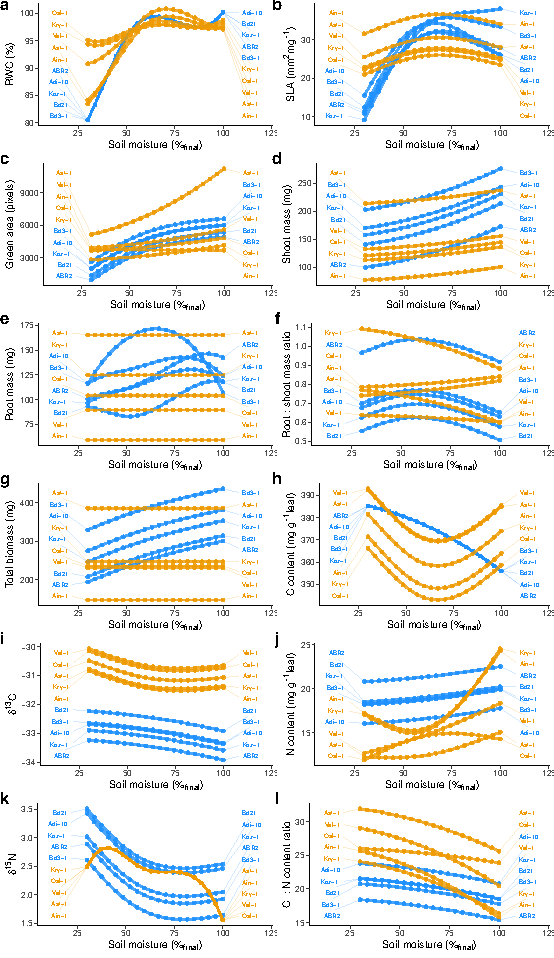
\includegraphics[width=\textwidth]{../Figures/curves_byspecies} \caption{\textbf{Variation in phenotypic responses to soil moisture gradient as function-valued traits.} \emph{B. sylvaticum} genotypes are colored orange and \emph{B. distachyon} blue. (a) RWC (b) SLA (c) Green Area (d) Shoot Mass (e) Root Mass (f) Root:Shoot (g) Biomass (h) C content (i) d13c (j) N content (k) d15n (l) C:N ratio}\label{fig:curves}
\end{figure}



\begin{figure*}[!h]
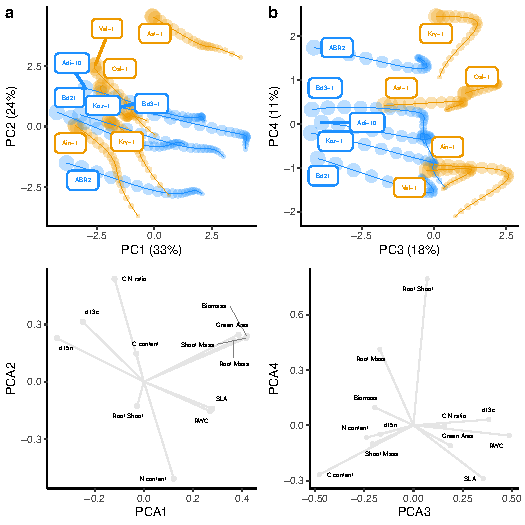
\includegraphics[width=\textwidth]{../Figures/pca_byspecies} \caption{\textbf{Plasticity through multivariate trait space.} (A) Plasticity across all traits was calculated as distance between scaled phenotype for each genotype between different levels of soil moisture. Box plots indicate species median and 25th and 75th percentiles with whiskers extending to 1.5 times the interquartile range. "*" indicates significant differences between species (t-test, \(\alpha < 0.05\)). Principal component analysis of scaled phenotypic responses to soil moisture gradient among genotypes of both species. Upper panels show genotype means across soil mositure content. Percent values in axis titles indicate percent variance explained by that principal component. Lower panels show eigenvectors of each trait. (B) PC1 and PC2. (C) PC3 and PC4.}\label{fig:pca}
\end{figure*}

\hypertarget{nearly-all-traits-show-significant-genetic-variation}{%
\subsubsection{Nearly all traits show significant genetic variation}\label{nearly-all-traits-show-significant-genetic-variation}}

We also tested whether there was significant natural variation for the traits measured between genotypes in each species by looking at the parameters in the final model for each trait. Interestingly, in both species and for all traits except relative water content in \emph{B. sylvaticum} the final model included a significant genotype term, indicating significant differences between genotypes in magnitude of traits across all levels of soil moisture (Table \ref{tab:models}, Figure \ref{fig:curves}). For other traits there are clear distinctions between the two species. For example, \(\delta C_{13}\) was considerably higher in \emph{B. sylvaticum} (Figure \ref{fig:curves}). For SLA, while \emph{B. distachyon} showed a strong response to soil moisture, especially under the driest conditions, SLA in \emph{B. sylvaticum} was not responsive to soil moisture. In contrast, \emph{B. sylvaticum} appears to show a more dramatic response in leaf composition estimated by N content and C:N ratio.

\hypertarget{several-traits-show-interactions-between-genotype-and-non-linear-responses-to-the-environment}{%
\subsubsection{Several traits show interactions between genotype and non-linear responses to the environment}\label{several-traits-show-interactions-between-genotype-and-non-linear-responses-to-the-environment}}

Significant interactions between genotype and environmental parameters in a final model indicate the presence of genetic variation for plasticity (GxE) (Via and Lande 1985). For those GxE interactions where the environmental parameter is non-linear, significant GxE indicates genetic variation for the shape of reaction norms. SLA showed a significant interaction between genotype and soil moisture in \emph{B. distachyon}. In \emph{B. sylvaticum}, nitrogen content, carbon to nitrogen ratio, above ground green area, and root to shoot ratio all showed significant interactions between genotype and soil moisture (Table \ref{tab:models}, Figure \ref{fig:curves}). In each of these cases, the interaction between genotype and environment involved a non-linear environmental predictor, indicating not only variation for the magnitude of plasticity (i.e.~slope) but also variation in the shape of responses.



\begin{figure*}[!h]
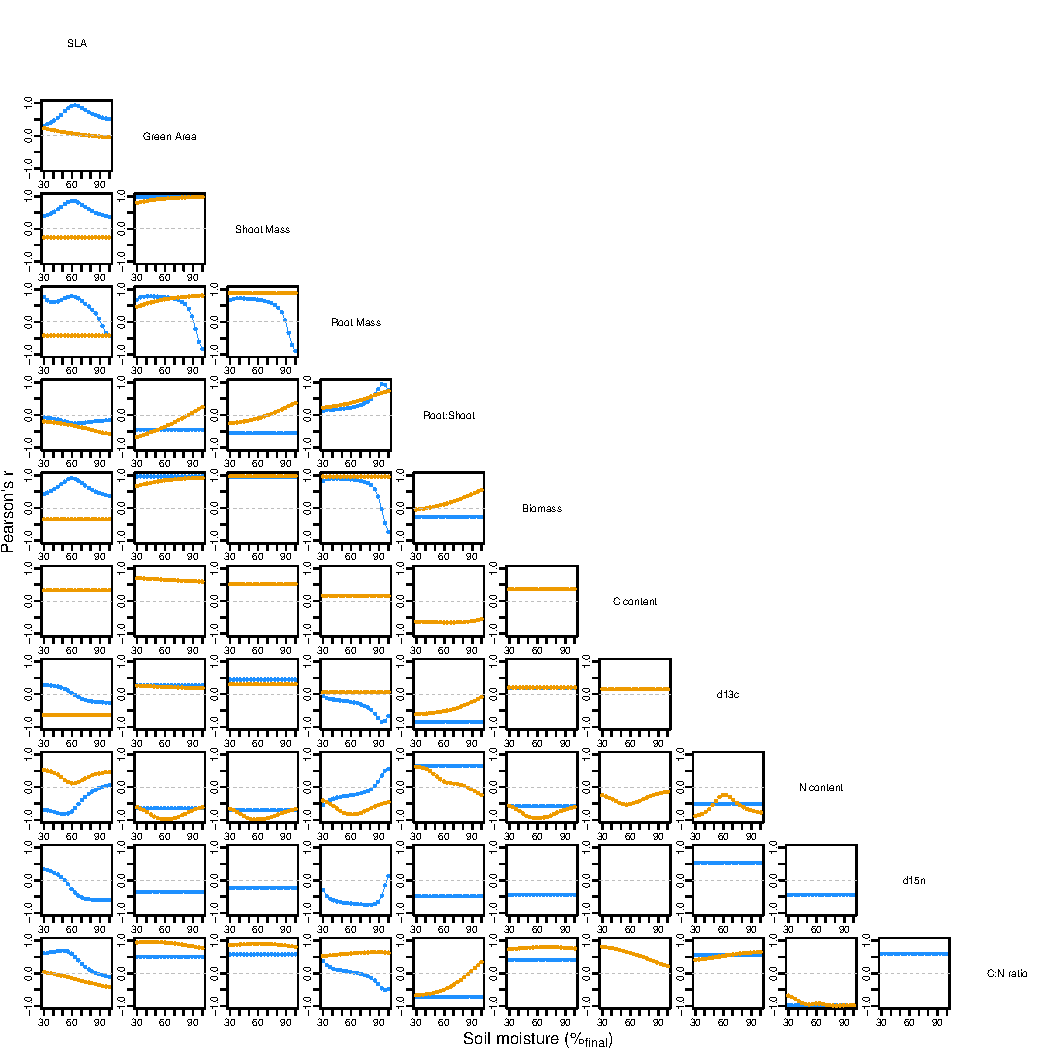
\includegraphics[width=\textwidth]{../Figures/corsplots_byspecies} \caption{\textbf{Trait correlations as a function of soil moisture content.} Correlations were calculated among genotypes by species (blue = \emph{B. distachyon}, orange = \emph{B. sylvaticum}). Note that correlations are not shown for traits in species where genotype was not included in final model (Table 1).}\label{fig:cors}
\end{figure*}



\begin{figure}[!h]
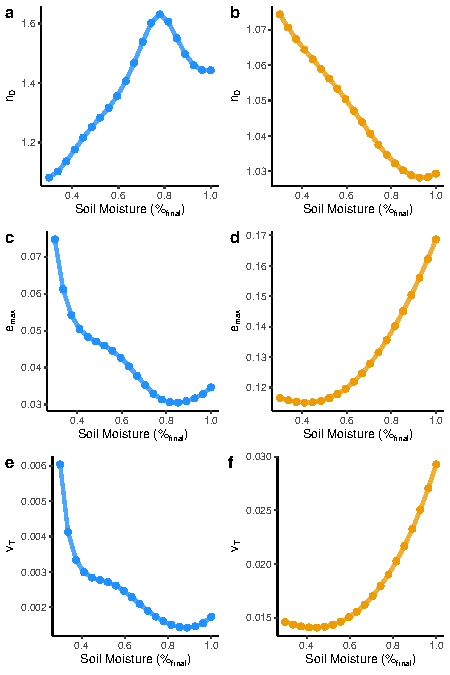
\includegraphics[width=\textwidth]{../Figures/constraints_byspecies} \caption{\textbf{Contrasting patterns of evolutionary constraint between \emph{B. distachyon} and \emph{B. sylvaticum}.} Summary statistics of evolutionary constraint as a function of soil moisture in \emph{B. distachyon} (blue) and \emph{B. sylvaticum} (orange). (a and b) The number of effective dimensions, \(n_D\), estimates number of unconstrained axes of variation (c and d) The maximum evolvability, \(e_{max}\), corresponds to the square root of the largest eigenvalue of the genetic covariance matrix. (e and f) The total genetic variance, \(v_T\), is equal to the sum of the eigenvalues of the genetic covariance matrix.}\label{fig:constraints}
\end{figure}

\hypertarget{correlations-between-traits-change-as-a-function-of-soil-moisture-often-in-a-non-linear-fashion}{%
\subsubsection{Correlations between traits change as a function of soil moisture, often in a non-linear fashion}\label{correlations-between-traits-change-as-a-function-of-soil-moisture-often-in-a-non-linear-fashion}}

We examined correlations between genotype trait means across soil moisture for traits where genotypic differences were observed (i.e.~genotype predictor in trait models). Certain traits were strongly correlated regardless of environment. For example, correlations near 1 were observed between biomass and green area in both species across soil moisture. More complex relationships between trait correlations and soil moisture are observed in other trait combinations. For traits with genotype by non-linear environment interactions (Table \ref{tab:models}), trait correlations showed non-linear relationships with soil moisture as well. Because more of these interactions were found in \emph{B. sylvaticum} the number of trait combinations showing non-linear relations between correlations and soil moisture appears to be higher than in \emph{B. distachyon} (Figure \ref{fig:cors}). In some cases, the relationship between soil moisture and trait correlation was dramatic. The correlation between C:N ratio and root:shoot ratio in \emph{B. sylvaticum}, for example, varied from approximately 0.3 under the wettest environment to approximately -0.7 under the driest environment.

\hypertarget{evolutionary-constraints-differ-as-a-function-of-soil-moisture-and-show-contrasting-patterns-between-brachypodium-species}{%
\subsubsection{\texorpdfstring{Evolutionary constraints differ as a function of soil moisture and show contrasting patterns between \emph{Brachypodium} species}{Evolutionary constraints differ as a function of soil moisture and show contrasting patterns between Brachypodium species}}\label{evolutionary-constraints-differ-as-a-function-of-soil-moisture-and-show-contrasting-patterns-between-brachypodium-species}}

To assess evidence of evolutionary constraint on the sampled traits, we estimated and analyzed parameters of the genetic covariance matrix, \(G\), in each species across the soil moisture gradient. These analyses revealed contrasting patterns of evolutionary constraint both in relation to soil moisture and between \emph{B. distachyon} and \emph{B. sylvaticum}. In \emph{B. distachyon}, the number of effective dimensions (\(n_D\), which estimates number of axes of variation unconstrained by covariance) was lower when soils were drier. In contrast, \(n_D\) was lower in \emph{B. sylvaticum} when soils were wetter. The maximum evolvability (\(e_{max}\), variance through largest eigenvector of multidimensional trait space) also showed opposite trends between the two species. Whereas in \emph{B. distachyon} \(e_{max}\) was highest under the driest conditions, in \emph{B. sylvaticum} \(e_{max}\) was highest under the wettest conditions. The same trend was seen in total genetic variance (\(V_T\), which summarizes all genetic variance through multidimensional trait space). These results indicate that \emph{B. distachyon} has increased genetic variance under dry conditions as compared to wet conditions, but that natural selection may be more constrained to act on this variation due to covariance between traits. In contrast, our results suggest that \emph{B. sylvaticum} has decreased genetic variance under dry conditions on which selection might act but that this variation is less constrained by covariance between traits.

\hypertarget{discussion}{%
\section{Discussion}\label{discussion}}

Environmental conditions vary along continuous gradients in space, time, and degree. Natural populations of organisms may therefore be exposed to a range of values for any particular dimension of the environment. The efficacy of natural selection to shape evolutionary response of populations depends on the magnitude of genetic variation in response to these environmental gradients and on the genetic correlation between traits as a function of the environment. Here, we explicitly model trait variation in two plant species as a continuous function of soil water availability and consider how genetic variance and co-variance in these functional responses may affect the evolution of plant-environment interaction.

\hypertarget{non-linearity-in-soil-moisture-response-is-pervasive-in-brachypodium}{%
\subsubsection{\texorpdfstring{Non-linearity in soil moisture response is pervasive in \emph{Brachypodium}}{Non-linearity in soil moisture response is pervasive in Brachypodium}}\label{non-linearity-in-soil-moisture-response-is-pervasive-in-brachypodium}}

We found significant non-linearity in response to a soil moisture gradient for all measured traits in at least one of the two species sampled. The best-fit function for some traits was quadratic, while other traits showed more complex responses to the environment which were best fit by a spline function. These results offer new insights with respect to the study of plant response to soil drying. By focusing on the curvature of phenotypic response as the explicitly modeled trait, we avoid contrasts of trait values expressed at arbitrary levels of soil water content which may obscure different thresholds of response among the diverse genotypes under study. SLA in \emph{B. distachyon} exhibits this pattern, as two accessions show a threshold-like response in decreasing SLA as soils become drier, and three accessions express their highest SLA at intermediate SWC. Leaf N content (on a leaf-mass basis) in \emph{B. sylvaticum} likewise shows considerable diversity of response with two accessions expressing their lowest values at intermediate SWC, one accession expressing its highest Leaf N at intermediate SWC, and one accession showing a nearly linear response along the SWC gradient.

\hypertarget{implications-for-evolution-of-brachypodium}{%
\subsubsection{\texorpdfstring{Implications for evolution of \emph{Brachypodium}}{Implications for evolution of Brachypodium}}\label{implications-for-evolution-of-brachypodium}}

Leaf N and SLA are two axes of the classic Leaf Economic Spectrum (Wright \emph{et al.} 2004) and so the contrasting responses of these traits between the annual \emph{B. distachyon} and perennial \emph{B. sylvaticum} may reflect broader differences in their life history strategies. We recently reviewed evidence for physiological, anatomical and developmental differences between herbaceous annual and perennial species, finding support for generally higher SLA in annuals, befitting a generally resource-acquisitive strategy (Lundgren and Des Marais). Garnier (Garnier 1992) argued that small changes in leaf anatomy (e.g.~SLA) will likely have large effects on plant growth rate and resource use and could therefore tip the balance between perennial and annual strategies.
We also found that signatures of evolutionary constraint differ along our imposed soil water content gradient. Specifically, we find evidence of highest evolvability in multitrait space (measured by \(e_{max}\) and \(v_T\)) in \emph{B. distachyon} under the driest soils. In contrast, \emph{B. sylvaticum} exhibited evidence of greater evolvability by the same measures under the highest soil water content studied here. We speculate that the pattern observed could be a reflection of the different life history strategies of these two species. Annuality is considered a drought adaptive strategy characterized by escaping drought through phenology, by flowering before and remaining dormant as seeds during the most drought prone seasons (Friedman and Rubin 2015; Monroe \emph{et al.} 2019) Thus, because of their life history, populations of annuals may actually experience fewer episodes of strong selection from extreme drought, which could explain why we find elevated genetic variance under these environments. In contrast, perennials such as \emph{B. sylvaticum} are subjected to all seasons and might therefore, experience more frequent episodes of selection caused by dehydration stress, despite paradoxically being in found in environments where droughts are less frequent on an annual basis. This pattern is consistent with the predictions of cryptic genetic variation revealed under environments where selection is less frequent or severe (Schlichting 2008).

\hypertarget{implications-for-breeding-drought-adaptation}{%
\subsubsection{Implications for breeding drought adaptation}\label{implications-for-breeding-drought-adaptation}}

We found that genetic correlations between traits can vary dramatically even over relatively small changes in soil moisture (Fig. \ref{fig:cors}). Responses to selection for drought tolerance may therefore depend on drought severity because of these patterns in genetic correlations. In the context of breeding, exploratory studies such as this may be valuable for identifying conditions for which genetic correlations are aligned with breeding objectives. Similarly, we found that signatures of evolutionary constraint varied across the environmental gradient, suggesting that responses to selection may be improved or restricted in accordance with patterns of constraint in relation to environment. Interestingly, we also found that some species may be more responsive to selection in a given environment based on patterns of constraint.

From a practical perspective this work highlights the value of function-valued trait approaches that may be extended to studying plant-water relations in agricultural settings. In this experiment, we investigated variation in plant responses to a gradient of soil moisture using six watering levels, which in combination with random variation in water capacity of experimental pots, produced a continuous gradient of soil moisture ranging from field capacity of the soil to strongly water-limited. In the field, multiple watering regimes in combination with random variability between plots may produce similar gradients of soil moisture. In this experiment, water content was measured gravimetrically. New sensing technologies may be useful for quantifying soil moisture in an analogous fashion, to define soil moisture quantitatively and then apply function-valued statistical approaches to contrast trait expression among genotypes.

\hypertarget{concluding-remarks}{%
\subsubsection{Concluding remarks}\label{concluding-remarks}}

Describing traits and their complex relationships with environmental and genetic variation continue to be challenges for biology. This goal is worthy of further effort if we are to address the challenges posed by climate change and understand organism evolution. Fortunately, new approaches such as analyses of function-valued traits and multivariate trait covariance analyses facilitate new discoveries. We hope that this study, by demonstrating the use of these approaches to yield novel insight into the influence of environment on phenotypes, trait correlations, and evolutionary constraint, will inspire further work to tackle the challenge of studying organisms and environments.

\hypertarget{acknowledgements}{%
\section{Acknowledgements}\label{acknowledgements}}

We thank Chase Mason and Eric Goolsby for insightful conversations about function-valued trait approaches. This work was supported by an Eco-Evo-Devo Network training grant to JGM.

\hypertarget{contributions}{%
\section{Contributions}\label{contributions}}

JGM and DD funded, planned, and conducted the experiment. JGM, HC, and DD contributed to analyses and writing.

\newpage

\begingroup
\setlength{\parindent}{-0.5in}
\setlength{\leftskip}{0.5in}

\hypertarget{refs}{}
\leavevmode\hypertarget{ref-blows2007tale}{}%
Blows M. W., 2007 A tale of two matrices: Multivariate approaches in evolutionary biology. Journal of evolutionary biology 20: 1--8.

\leavevmode\hypertarget{ref-brkljacic2011brachypodium}{}%
Brkljacic J., E. Grotewold, R. Scholl, T. Mockler, and D. F. Garvin \emph{et al.}, 2011 Brachypodium as a model for the grasses: Today and the future. Plant Physiology 157: 3--13.

\leavevmode\hypertarget{ref-brommer2008exploring}{}%
Brommer J. E., K. Rattiste, and A. J. Wilson, 2008 Exploring plasticity in the wild: Laying date--temperature reaction norms in the common gull larus canus. Proceedings of the Royal Society B: Biological Sciences 275: 687--693.

\leavevmode\hypertarget{ref-casper2001drought}{}%
Casper B., I. Forseth, H. Kempenich, S. Seltzer, and K. Xavier, 2001 Drought prolongs leaf life span in the herbaceous desert perennial cryptantha flava. Functional Ecology 15: 740--747.

\leavevmode\hypertarget{ref-catalan2016phylogeny}{}%
Catalan P., D. Lopez-Alvarez, A. Diaz-Perez, R. Sancho, and M. L. Lopez-Herranz, 2016 Phylogeny and evolution of the genus brachypodium, in \emph{Genetics and genomics of brachypodium}, Plant genetics and genomics: Crop models. edited by Vogel J. Springer International.

\leavevmode\hypertarget{ref-des2012physiological}{}%
Des Marais D. L., J. K. McKay, J. H. Richards, S. Sen, and T. Wayne \emph{et al.}, 2012 Physiological genomics of response to soil drying in diverse arabidopsis accessions. The Plant Cell 24: 893--914.

\leavevmode\hypertarget{ref-des2017interactive}{}%
Des Marais D. L., J. R. Lasky, P. E. Verslues, T. Z. Chang, and T. E. Juenger, 2017 Interactive effects of water limitation and elevated temperature on the physiology, development and fitness of diverse accessions of brachypodium distachyon. New Phytologist 214: 132--144.

\leavevmode\hypertarget{ref-dittberner2018natural}{}%
Dittberner H., A. Korte, T. Mettler-Altmann, A. P. Weber, and G. Monroe \emph{et al.}, 2018 Natural variation in stomata size contributes to the local adaptation of water-use efficiency in arabidopsis thaliana. Molecular ecology 27: 4052--4065.

\leavevmode\hypertarget{ref-edwards2012quantitative}{}%
Edwards C. E., B. E. Ewers, C. R. McClung, P. Lou, and C. Weinig, 2012 Quantitative variation in water-use efficiency across water regimes and its relationship with circadian, vegetative, reproductive, and leaf gas-exchange traits. Molecular Plant 5: 653--668.

\leavevmode\hypertarget{ref-el2014genotype}{}%
El-Soda M., M. P. Boer, H. Bagheri, C. J. Hanhart, and M. Koornneef \emph{et al.}, 2014 Genotype--environment interactions affecting preflowering physiological and morphological traits of brassica rapa grown in two watering regimes. Journal of experimental botany 65: 697--708.

\leavevmode\hypertarget{ref-friedman2015all}{}%
Friedman J., and M. J. Rubin, 2015 All in good time: Understanding annual and perennial strategies in plants. American journal of botany 102: 497--499.

\leavevmode\hypertarget{ref-garnier1992growth}{}%
Garnier E., 1992 Growth analysis of congeric annual and perennial grass species. Journal of Ecology 80: 665--675.

\leavevmode\hypertarget{ref-gomulkiewicz2018variation}{}%
Gomulkiewicz R., J. G. Kingsolver, P. A. Carter, and N. Heckman, 2018 Variation and evolution of function-valued traits. Annual Review of Ecology, Evolution, and Systematics 49: 139--164.

\leavevmode\hypertarget{ref-goolsby2015phylogenetic}{}%
Goolsby E. W., 2015 Phylogenetic comparative methods for evaluating the evolutionary history of function-valued traits. Systematic biology 64: 568--578.

\leavevmode\hypertarget{ref-greenham2017temporal}{}%
Greenham K., C. R. Guadagno, M. A. Gehan, T. C. Mockler, and C. Weinig \emph{et al.}, 2017 Temporal network analysis identifies early physiological and transcriptomic indicators of mild drought in brassica rapa. Elife 6: e29655.

\leavevmode\hypertarget{ref-griswold2008hypothesis}{}%
Griswold C. K., R. Gomulkiewicz, and N. Heckman, 2008 Hypothesis testing in comparative and experimental studies of function-valued traits. Evolution 62: 1229--1242.

\leavevmode\hypertarget{ref-houle1992comparing}{}%
Houle D., 1992 Comparing evolvability and variability of quantitative traits. Genetics 130: 195--204.

\leavevmode\hypertarget{ref-juenger2013natural}{}%
Juenger T. E., 2013 Natural variation and genetic constraints on drought tolerance. Current opinion in plant biology 16: 274--281.

\leavevmode\hypertarget{ref-kesari2012intron}{}%
Kesari R., J. R. Lasky, J. G. Villamor, Des MaraisD. L., and Y.-J. C. Chen \emph{et al.}, 2012 Intron-mediated alternative splicing of arabidopsis p5cs1 and its association with natural variation in proline and climate adaptation. Proceedings of the National Academy of Sciences 109: 9197--9202.

\leavevmode\hypertarget{ref-kingsolver2001variation}{}%
Kingsolver J. G., R. Gomulkiewicz, and P. A. Carter, 2001 Variation, selection and evolution of function-valued traits, pp. 87--104 in \emph{Microevolution rate, pattern, process}, Springer.

\leavevmode\hypertarget{ref-kingsolver2003environmental}{}%
Kingsolver J. G., and R. Gomulkiewicz, 2003 Environmental variation and selection on performance curves. Integrative and Comparative Biology 43: 470--477.

\leavevmode\hypertarget{ref-kingsolver2015genetic}{}%
Kingsolver J. G., N. Heckman, J. Zhang, P. A. Carter, and J. L. Knies \emph{et al.}, 2015 Genetic variation, simplicity, and evolutionary constraints for function-valued traits. The American Naturalist 185: E166--E181.

\leavevmode\hypertarget{ref-kirkpatrick1989quantitative}{}%
Kirkpatrick M., and N. Heckman, 1989 A quantitative genetic model for growth, shape, reaction norms, and other infinite-dimensional characters. Journal of mathematical biology 27: 429--450.

\leavevmode\hypertarget{ref-kirkpatrick2009patterns}{}%
Kirkpatrick M., 2009 Patterns of quantitative genetic variation in multiple dimensions. Genetica 136: 271--284.

\leavevmode\hypertarget{ref-lenk2019transcriptional}{}%
Lenk I., L. H. C. Fisher, M. Vickers, A. Akinyemi, and T. Didion \emph{et al.}, 2019 Transcriptional and metabolomic analyses indicate that cell wall properties are associated with drought tolerance in brachypodium distachyon. Int J Mol Sci 20. \url{https://doi.org/10.3390/ijms20071758}

\leavevmode\hypertarget{ref-levins1968evolution}{}%
Levins R., 1968 \emph{Evolution in changing environments: Some theoretical explorations}. Princeton University Press.

\leavevmode\hypertarget{ref-lundgren2020lifehistory}{}%
Lundgren M. R., and Des MaraisD. L., Life history variation as a model for understanding trade-offs in plant-environment interactions. Current Biology.

\leavevmode\hypertarget{ref-luo2016specific}{}%
Luo N., X. Yu, G. Nie, J. Liu, and Y. Jiang, 2016 Specific peroxidases differentiate brachypodium distachyon accessions and are associated with drought tolerance traits. Ann Bot 118: 259--70. \url{https://doi.org/10.1093/aob/mcw104}

\leavevmode\hypertarget{ref-mason2020learning}{}%
Mason C. M., M. C. LaScaleia, De La PascuaD. R., J. G. Monroe, and E. W. Goolsby, 2020 Learning from dynamic traits: Seasonal shifts yield insights into ecophysiological trade-offs across scales from macroevolutionary to intraindividual. International Journal of Plant Sciences 181: 88--102.

\leavevmode\hypertarget{ref-mcguigan2009condition}{}%
McGuigan K., 2009 Condition dependence varies with mating success in male drosophila bunnanda. Journal of evolutionary biology 22: 1813--1825.

\leavevmode\hypertarget{ref-mcguigan2010quantitative}{}%
McGuigan K., N. Nishimura, M. Currey, D. Hurwit, and W. A. Cresko, 2010 Quantitative genetic variation in static allometry in the threespine stickleback. Integrative and comparative biology 50: 1067--1080.

\leavevmode\hypertarget{ref-meyer2005randomregression}{}%
Meyer K., 2005 Random regression analyses using b-splines to model growth of australian angus cattle. Genet. Sel. Evol. 37: 473--500.

\leavevmode\hypertarget{ref-monroe2019drought}{}%
Monroe J. G., B. Gill, K. G. Turner, and J. K. McKay, 2019 Drought regimens predict life history strategies in heliophila. New Phytologist 223: 2054--2062.

\leavevmode\hypertarget{ref-passioura1996drought}{}%
Passioura J., 1996 Drought and drought tolerance. Plant growth regulation 20: 79--83.

\leavevmode\hypertarget{ref-pearse2019life}{}%
Pearse I. S., J. M. Aguilar, and S. Y. Strauss, 2019 Life history plasticity and water use trade-offs associated with drought resistance in a clade of california jewelflowers

\leavevmode\hypertarget{ref-pettay2008age}{}%
Pettay J. E., A. Charmantier, A. J. Wilson, and V. Lummaa, 2008 Age-specific genetic and maternal effects in fecundity of preindustrial finnish women. Evolution: International Journal of Organic Evolution 62: 2297--2304.

\leavevmode\hypertarget{ref-robinson2009impact}{}%
Robinson M. R., A. J. Wilson, J. G. Pilkington, T. H. Clutton-Brock, and J. M. Pemberton \emph{et al.}, 2009 The impact of environmental heterogeneity on genetic architecture in a wild population of soay sheep. Genetics 181: 1639--1648.

\leavevmode\hypertarget{ref-rocha2012connecting}{}%
Rocha F. B., and L. B. Klaczko, 2012 Connecting the dots of nonlinear reaction norms unravels the threads of genotype--environment interaction in drosophila. Evolution: International Journal of Organic Evolution 66: 3404--3416.

\leavevmode\hypertarget{ref-schlichting2008hidden}{}%
Schlichting C. D., 2008 Hidden reaction norms, cryptic genetic variation, and evolvability. Annals of the New York Academy of Sciences 1133: 187--203.

\leavevmode\hypertarget{ref-skirycz2011pause}{}%
Skirycz A., H. Claeys, De BodtS., A. Oikawa, and S. Shinoda \emph{et al.}, 2011 Pause-and-stop: The effects of osmotic stress on cell proliferation during early leaf development in arabidopsis and a role for ethylene signaling in cell cycle arrest. Plant Cell 23: 1876--88. \url{https://doi.org/10.1105/tpc.111.084160}

\leavevmode\hypertarget{ref-steinwand2013sylvaticum}{}%
Steinwand M. A., H. A. Young, J. N. Bragg, C. M. Tobias, and J. P. Vogel, 2013 Brachypodium sylvaticum, a model for perennial grasses: Transformation and inbred line development. PLoS One 8: e75180. \url{https://doi.org/10.1371/journal.pone.0075180}

\leavevmode\hypertarget{ref-stinchcombe2010across}{}%
Stinchcombe J. R., R. Izem, M. S. Heschel, B. V. McGoey, and J. Schmitt, 2010 Across-environment genetic correlations and the frequency of selective environments shape the evolutionary dynamics of growth rate in impatiens capensis. Evolution: International Journal of Organic Evolution 64: 2887--2903.

\leavevmode\hypertarget{ref-stinchcombe2012genetics}{}%
Stinchcombe J. R., M. Kirkpatrick, F.-v. T. W. Group, and others, 2012 Genetics and evolution of function-valued traits: Understanding environmentally responsive phenotypes. Trends in Ecology \& Evolution 27: 637--647.

\leavevmode\hypertarget{ref-vasseur2014multivariate}{}%
Vasseur F., T. Bontpart, M. Dauzat, C. Granier, and D. Vile, 2014 Multivariate genetic analysis of plant responses to water deficit and high temperature revealed contrasting adaptive strategies. Journal of experimental botany 65: 6457--6469.

\leavevmode\hypertarget{ref-MASS}{}%
Venables W. N., and B. D. Ripley, 2002 \emph{Modern applied statistics with s}. Springer, New York.

\leavevmode\hypertarget{ref-verelst2013molecular}{}%
Verelst W., E. Bertolini, De BodtS., K. Vandepoele, and M. Demeulenaere \emph{et al.}, 2013 Molecular and physiological analysis of growth-limiting drought stress in brachypodium distachyon leaves. Mol Plant 6: 311--22. \url{https://doi.org/10.1093/mp/sss098}

\leavevmode\hypertarget{ref-verslues2011drought}{}%
Verslues P. E., and T. E. Juenger, 2011 Drought, metabolites, and arabidopsis natural variation: A promising combination for understanding adaptation to water-limited environments. Current opinion in plant biology 14: 240--245.

\leavevmode\hypertarget{ref-via1985genotype}{}%
Via S., and R. Lande, 1985 Genotype-environment interaction and the evolution of phenotypic plasticity. Evolution 39: 505--522.

\leavevmode\hypertarget{ref-vogel2009development}{}%
Vogel J. P., M. Tuna, H. Budak, N. Huo, and Y. Q. Gu \emph{et al.}, 2009 Development of ssr markers and analysis of diversity in turkish populations of brachypodium distachyon. BMC Plant Biology 9: 88.

\leavevmode\hypertarget{ref-wright2004worldwide}{}%
Wright I. J., P. B. Reich, M. Westoby, D. D. Ackerly, and Z. Baruch \emph{et al.}, 2004 The worldwide leaf economics spectrum. Nature 428: 821.

\leavevmode\hypertarget{ref-yarkhunova2016selection}{}%
Yarkhunova Y., C. E. Edwards, B. E. Ewers, R. L. Baker, and T. L. Aston \emph{et al.}, 2016 Selection during crop diversification involves correlated evolution of the circadian clock and ecophysiological traits in brassica rapa. New Phytologist 210: 133--144.

\endgroup

\newpage
\setcounter{table}{0}  \renewcommand{\thetable}{S\arabic{table}} \setcounter{figure}{0} \renewcommand{\thefigure}{S\arabic{figure}}

\hypertarget{supplement}{%
\section{Supplement}\label{supplement}}

\begin{table*}[tbp]
\begin{center}
\begin{threeparttable}
\caption{\label{tab:outmodels}final models}
\tiny{
\begin{tabular}{lllllll}
\toprule
 & \multicolumn{1}{c}{Df} & \multicolumn{1}{c}{Sum.Sq} & \multicolumn{1}{c}{Mean.Sq} & \multicolumn{1}{c}{F.value} & \multicolumn{1}{c}{Pr..F.} & \multicolumn{1}{c}{trait}\\
\midrule
I(Day\_14\textasciicircum{}2) & 1.00000 & 1,749.17374 & 1,749.17374 & 113.13775 & 0.00000 & Relative\_WC b\_dist\\
ns(Day\_14,df=2) & 2.00000 & 1,875.17736 & 937.58868 & 60.64387 & 0.00000 & Relative\_WC b\_dist\\
Harv & 4.00000 & 205.30059 & 51.32515 & 3.31975 & 0.01248 & Relative\_WC b\_dist\\
Residuals & 137.00000 & 2,118.09770 & 15.46057 & NA & NA & Relative\_WC b\_dist\\
Geno & 4.00000 & 323.29367 & 80.82342 & 3.39597 & 0.01138 & Relative\_WC b\_sylv\\
ns(Day\_14,df=2)1 & 2.00000 & 671.68506 & 335.84253 & 14.11116 & 0.00000 & Relative\_WC b\_sylv\\
Harv1 & 4.00000 & 268.15302 & 67.03826 & 2.81676 & 0.02817 & Relative\_WC b\_sylv\\
Residuals1 & 121.00000 & 2,879.77449 & 23.79979 & NA & NA & Relative\_WC b\_sylv\\
Geno1 & 4.00000 & 140.92870 & 35.23217 & 1.75884 & 0.14122 & SLA b\_dist\\
I(Day\_14\textasciicircum{}2)1 & 1.00000 & 2,414.64758 & 2,414.64758 & 120.54272 & 0.00000 & SLA b\_dist\\
ns(Day\_14,df=2)2 & 2.00000 & 2,327.88690 & 1,163.94345 & 58.10575 & 0.00000 & SLA b\_dist\\
Harv2 & 4.00000 & 651.79297 & 162.94824 & 8.13461 & 0.00001 & SLA b\_dist\\
GenoI(Day\_14\textasciicircum{}2) & 4.00000 & 337.42496 & 84.35624 & 4.21119 & 0.00310 & SLA b\_dist\\
Residuals2 & 127.00000 & 2,543.99629 & 20.03147 & NA & NA & SLA b\_dist\\
Geno2 & 4.00000 & 1,572.00031 & 393.00008 & 12.05355 & 0.00000 & SLA b\_sylv\\
ns(Day\_14,df=2)3 & 2.00000 & 162.19048 & 81.09524 & 2.48724 & 0.08735 & SLA b\_sylv\\
Residuals3 & 122.00000 & 3,977.75094 & 32.60452 & NA & NA & SLA b\_sylv\\
Geno3 & 4.00000 & 32,376,338.95160 & 8,094,084.73790 & 5.44806 & 0.00043 & aboveground\_greenarea b\_dist\\
ns(Day\_14,df=2)4 & 2.00000 & 192,517,942.01652 & 96,258,971.00826 & 64.79115 & 0.00000 & aboveground\_greenarea b\_dist\\
Harv3 & 4.00000 & 59,381,207.50609 & 14,845,301.87652 & 9.99225 & 0.00000 & aboveground\_greenarea b\_dist\\
Residuals4 & 134.00000 & 199,081,240.28441 & 1,485,680.89764 & NA & NA & aboveground\_greenarea b\_dist\\
Geno4 & 4.00000 & 219,846,397.86896 & 54,961,599.46724 & 15.60576 & 0.00000 & aboveground\_greenarea b\_sylv\\
I(Day\_14\textasciicircum{}2)2 & 1.00000 & 24,060,407.68683 & 24,060,407.68683 & 6.83170 & 0.01005 & aboveground\_greenarea b\_sylv\\
Harv4 & 4.00000 & 77,050,113.87350 & 19,262,528.46838 & 5.46939 & 0.00043 & aboveground\_greenarea b\_sylv\\
GenoI(Day\_14\textasciicircum{}2)1 & 4.00000 & 33,700,623.60514 & 8,425,155.90129 & 2.39223 & 0.05412 & aboveground\_greenarea b\_sylv\\
Residuals5 & 126.00000 & 443,756,646.65128 & 3,521,878.14803 & NA & NA & aboveground\_greenarea b\_sylv\\
Geno5 & 4.00000 & 151,815.09343 & 37,953.77336 & 17.16469 & 0.00000 & Shoot\_Mass b\_dist\\
I(Day\_14\textasciicircum{}2)3 & 1.00000 & 66,562.14458 & 66,562.14458 & 30.10291 & 0.00000 & Shoot\_Mass b\_dist\\
Harv5 & 4.00000 & 102,805.02689 & 25,701.25672 & 11.62346 & 0.00000 & Shoot\_Mass b\_dist\\
Residuals6 & 136.00000 & 300,716.87291 & 2,211.15348 & NA & NA & Shoot\_Mass b\_dist\\
Geno6 & 4.00000 & 282,513.50822 & 70,628.37705 & 24.41054 & 0.00000 & Shoot\_Mass b\_sylv\\
I(Day\_14\textasciicircum{}2)4 & 1.00000 & 6,122.54739 & 6,122.54739 & 2.11607 & 0.14821 & Shoot\_Mass b\_sylv\\
Harv6 & 4.00000 & 50,339.74373 & 12,584.93593 & 4.34960 & 0.00248 & Shoot\_Mass b\_sylv\\
Residuals7 & 128.00000 & 370,349.46472 & 2,893.35519 & NA & NA & Shoot\_Mass b\_sylv\\
Geno7 & 4.00000 & 52,681.25005 & 13,170.31251 & 23.75364 & 0.00000 & Root\_Mass b\_dist\\
I(Day\_14\textasciicircum{}2)5 & 1.00000 & 13,857.56690 & 13,857.56690 & 24.99316 & 0.00000 & Root\_Mass b\_dist\\
ns(Day\_14,df=2)5 & 2.00000 & 2,853.05835 & 1,426.52918 & 2.57285 & 0.08032 & Root\_Mass b\_dist\\
Harv7 & 4.00000 & 6,739.85641 & 1,684.96410 & 3.03896 & 0.01976 & Root\_Mass b\_dist\\
Genons(Day\_14,df=2) & 8.00000 & 8,723.71652 & 1,090.46457 & 1.96673 & 0.05586 & Root\_Mass b\_dist\\
Residuals8 & 126.00000 & 69,861.25916 & 554.45444 & NA & NA & Root\_Mass b\_dist\\
Geno8 & 4.00000 & 176,944.42509 & 44,236.10627 & 24.22780 & 0.00000 & Root\_Mass b\_sylv\\
Residuals9 & 133.00000 & 242,836.80767 & 1,825.84066 & NA & NA & Root\_Mass b\_sylv\\
Geno9 & 4.00000 & 2.81680 & 0.70420 & 36.70369 & 0.00000 & Shoot\_Root\_Ratio b\_dist\\
ns(Day\_14,df=2)6 & 2.00000 & 0.15610 & 0.07805 & 4.06809 & 0.01925 & Shoot\_Root\_Ratio b\_dist\\
Harv8 & 4.00000 & 1.14490 & 0.28623 & 14.91840 & 0.00000 & Shoot\_Root\_Ratio b\_dist\\
Residuals10 & 135.00000 & 2.59012 & 0.01919 & NA & NA & Shoot\_Root\_Ratio b\_dist\\
Geno10 & 4.00000 & 2.15066 & 0.53767 & 58.14315 & 0.00000 & Shoot\_Root\_Ratio b\_sylv\\
I(Day\_14\textasciicircum{}2)6 & 1.00000 & 0.04624 & 0.04624 & 5.00027 & 0.02713 & Shoot\_Root\_Ratio b\_sylv\\
Harv9 & 4.00000 & 0.38527 & 0.09632 & 10.41571 & 0.00000 & Shoot\_Root\_Ratio b\_sylv\\
GenoI(Day\_14\textasciicircum{}2)2 & 4.00000 & 0.13787 & 0.03447 & 3.72728 & 0.00671 & Shoot\_Root\_Ratio b\_sylv\\
Residuals11 & 124.00000 & 1.14666 & 0.00925 & NA & NA & Shoot\_Root\_Ratio b\_sylv\\
Geno11 & 4.00000 & 312,787.50625 & 78,196.87656 & 18.62845 & 0.00000 & biomass b\_dist\\
ns(Day\_14,df=2)7 & 2.00000 & 147,377.96199 & 73,688.98099 & 17.55455 & 0.00000 & biomass b\_dist\\
Harv10 & 4.00000 & 145,877.82793 & 36,469.45698 & 8.68793 & 0.00000 & biomass b\_dist\\
Residuals12 & 135.00000 & 566,691.30055 & 4,197.71334 & NA & NA & biomass b\_dist\\
Geno12 & 4.00000 & 862,484.81413 & 215,621.20353 & 24.16680 & 0.00000 & biomass b\_sylv\\
Harv11 & 4.00000 & 98,371.42927 & 24,592.85732 & 2.75636 & 0.03065 & biomass b\_sylv\\
Residuals13 & 129.00000 & 1,150,964.71805 & 8,922.20712 & NA & NA & biomass b\_sylv\\
I(Day\_14\textasciicircum{}2)7 & 1.00000 & 9,393.36268 & 9,393.36268 & 4.44262 & 0.03680 & c\_content b\_dist\\
Residuals14 & 143.00000 & 302,355.81423 & 2,114.37632 & NA & NA & c\_content b\_dist\\
Geno13 & 4.00000 & 16,887.94249 & 4,221.98562 & 4.20111 & 0.00314 & c\_content b\_sylv\\
ns(Day\_14,df=2)8 & 2.00000 & 3,997.44433 & 1,998.72217 & 1.98884 & 0.14106 & c\_content b\_sylv\\
Residuals15 & 128.00000 & 128,635.92473 & 1,004.96816 & NA & NA & c\_content b\_sylv\\
Geno14 & 4.00000 & 14.72235 & 3.68059 & 24.76573 & 0.00000 & d13c b\_dist\\
I(Day\_14\textasciicircum{}2)8 & 1.00000 & 4.81710 & 4.81710 & 32.41303 & 0.00000 & d13c b\_dist\\
Harv12 & 4.00000 & 7.60700 & 1.90175 & 12.79639 & 0.00000 & d13c b\_dist\\
Residuals16 & 135.00000 & 20.06317 & 0.14862 & NA & NA & d13c b\_dist\\
Geno15 & 4.00000 & 12.87800 & 3.21950 & 14.09960 & 0.00000 & d13c b\_sylv\\
ns(Day\_14,df=2)9 & 2.00000 & 3.81605 & 1.90802 & 8.35607 & 0.00039 & d13c b\_sylv\\
Harv13 & 4.00000 & 25.16097 & 6.29024 & 27.54772 & 0.00000 & d13c b\_sylv\\
Residuals17 & 124.00000 & 28.31414 & 0.22834 & NA & NA & d13c b\_sylv\\
Geno16 & 4.00000 & 332.26225 & 83.06556 & 8.93282 & 0.00000 & n\_content b\_dist\\
I(Day\_14\textasciicircum{}2)9 & 1.00000 & 15.55323 & 15.55323 & 1.67259 & 0.19812 & n\_content b\_dist\\
Harv14 & 4.00000 & 139.69914 & 34.92478 & 3.75579 & 0.00626 & n\_content b\_dist\\
Residuals18 & 135.00000 & 1,255.35355 & 9.29892 & NA & NA & n\_content b\_dist\\
Geno17 & 4.00000 & 456.11421 & 114.02855 & 25.06977 & 0.00000 & n\_content b\_sylv\\
ns(Day\_14,df=2)10 & 2.00000 & 325.38436 & 162.69218 & 35.76872 & 0.00000 & n\_content b\_sylv\\
Genons(Day\_14,df=2)1 & 8.00000 & 145.98218 & 18.24777 & 4.01187 & 0.00030 & n\_content b\_sylv\\
Residuals19 & 120.00000 & 545.81385 & 4.54845 & NA & NA & n\_content b\_sylv\\
Geno18 & 4.00000 & 14.25665 & 3.56416 & 5.34810 & 0.00050 & d15n b\_dist\\
ns(Day\_14,df=2)11 & 2.00000 & 14.26839 & 7.13419 & 10.70500 & 0.00005 & d15n b\_dist\\
Harv15 & 4.00000 & 21.75070 & 5.43768 & 8.15934 & 0.00001 & d15n b\_dist\\
Residuals20 & 134.00000 & 89.30239 & 0.66644 & NA & NA & d15n b\_dist\\
I(Day\_14\textasciicircum{}2)10 & 1.00000 & 17.12283 & 17.12283 & 32.60495 & 0.00000 & d15n b\_sylv\\
ns(Day\_14,df=2)12 & 2.00000 & 2.16282 & 1.08141 & 2.05920 & 0.13179 & d15n b\_sylv\\
Harv16 & 4.00000 & 13.73616 & 3.43404 & 6.53903 & 0.00008 & d15n b\_sylv\\
Residuals21 & 127.00000 & 66.69536 & 0.52516 & NA & NA & d15n b\_sylv\\
Geno19 & 4.00000 & 434.41850 & 108.60463 & 18.40460 & 0.00000 & c\_n b\_dist\\
I(Day\_14\textasciicircum{}2)11 & 1.00000 & 79.87162 & 79.87162 & 13.53538 & 0.00034 & c\_n b\_dist\\
Harv17 & 4.00000 & 75.29789 & 18.82447 & 3.19007 & 0.01537 & c\_n b\_dist\\
Residuals22 & 135.00000 & 796.62842 & 5.90095 & NA & NA & c\_n b\_dist\\
Geno20 & 4.00000 & 1,484.86836 & 371.21709 & 40.40652 & 0.00000 & c\_n b\_sylv\\
I(Day\_14\textasciicircum{}2)12 & 1.00000 & 488.17121 & 488.17121 & 53.13683 & 0.00000 & c\_n b\_sylv\\
GenoI(Day\_14\textasciicircum{}2)3 & 4.00000 & 90.41398 & 22.60349 & 2.46036 & 0.04877 & c\_n b\_sylv\\
Residuals23 & 125.00000 & 1,148.38252 & 9.18706 & NA & NA & c\_n b\_sylv\\
\bottomrule
\end{tabular}
}
\end{threeparttable}
\end{center}
\end{table*}



\begin{figure*}[!h]
\includegraphics[width=\textwidth]{../Figures/maps} \caption{Distributions of (a) \emph{B. distachyon} and (b) \emph{B. sylvaticum} reported on GBIF as of 2019.18.08. Examples of (c) \emph{B. distachyon} Carly Slawson (CC BY 4.0, \url{https://www.inaturalist.org/photos/42532397}) and (d) \emph{B. sylvaticum} Grzegorz Grzejszczak (CC BY-NC 4.0, \url{https://www.inaturalist.org/photos/3608899}).}\label{fig:maps}
\end{figure*}



\begin{figure*}[!h]

\includegraphics[width=\textwidth]{../Figures/racks_IDs} \caption{Planting scheme.}\label{fig:racks}
\end{figure*}



\begin{figure*}[!h]
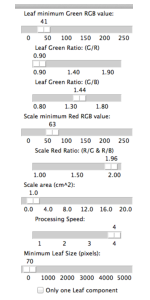
\includegraphics[width=\textwidth]{../Figures/settings_used} \caption{Settings used in Easy Leaf Area.}\label{fig:leafarea}
\end{figure*}



\begin{figure}[!h]
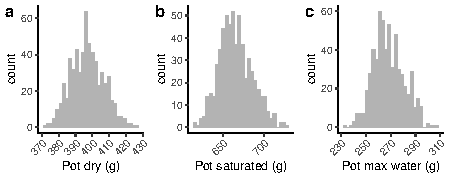
\includegraphics[width=\textwidth]{../Figures/pots} \caption{Variation in pot field capacity.}\label{fig:pots}
\end{figure}


\end{document}
